\chapter{Telescopi}

\section{Introduzione alle strutture dei telescopi e ai fenomeni ottici}

Per ora ci limiteremo a trattare i telescopi nella banda dell'ottico, anche se il discorso rimane molto simile anche per altre bande, essendo comunque basati sulla collezione di fotoni ad una certa lunghezza d'onda tramite riflessione su una superficie curva (processo di riflessione che risulta impossibile già con i raggi X). Le caratteristiche principali di un telescopio sono: sensibilità della misura (o flusso limite), potere risolutivo (ossia risoluzione angolare), campo di vista (o fov), larghezza di banda (determinata essenzialmente dallo strumento stesso), risoluzione spettrale.

\begin{wrapfigure}{r}{0.5\textwidth}
	%Immagine presa da slide
	\vspace{-10pt}
	\centering
	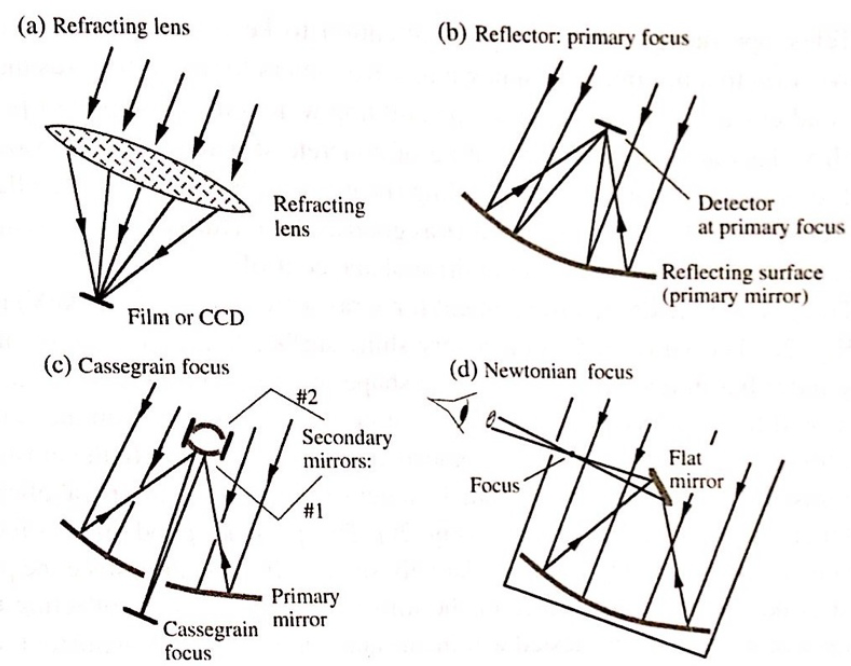
\includegraphics[width=0.49\textwidth]{./Immagini/Capitolo2/Telescopi_classici.png}
	\caption{Telescopi classici nell'ottico}
	\vspace{-10pt}
\end{wrapfigure}

Dal punto di vista storico, sin dai tempi di Galileo i primi telescopi funzionavano a rifrazione, è necessario aspettare Newton per vedere i primi telescopi a riflessione, inizialmente basati su specchi sferici poi cambiati in parabolici per ridurre le aberrazioni generate dai primi. Di quest'ultima tipologia di telescopi, il più semplice e immediato è quello in cui il focus primario è messo immediatamente sopra lo specchio principale. Un altro modello che venne adottato frequentemente è quello di \textbf{Cassegrain}, in cui il fascio è ridirezione da uno specchio secondario, posto nello stesso punto in cui si trova il focus nel modello precedente, con riflessione del fascio in un buco dello specchio primario, un altro modello è quello a focus laterale e così via. Il motivo per cui si sono superati i telescopi rifrattori, è perchè necessariamente il telescopio dovrebbe essere lungo almeno quanto la lunghezza focale della lente, creando una strumentazione particolarmente ingombrante e scomoda. Un altro fattore non trascurabile è quello per cui questo tipo di lenti portano a un'aberrazione non trascurabile, inoltre questo tipo di telescopio deve essere necessariamente chiuso, contenendo la lente, ma il fascio focalizzato deve quindi attraversare una zona chiusa che per gradienti termici può creare moti convettivi che vanno a intaccare la bontà dell'osservazione, evitabili con una struttura aperta possibile solo con telescopi riflettivi. Si ricorda che per proprietà delle lenti, la \textbf{aberrazione cromatica} è il fenomeno per cui una lente ha indici di rifrazione diversi per lunghezze d'onda diverse, ciò genera un gradiente di colore, il che significa che a lunghezze focali sufficientemente grandi si ottengono punti di focus diversi a seconda della lunghezza d'onda osservata, anche nella stessa banda. Il problema è risolvibile aggiungendo sistemi di lenti correttrici il cui compito è proprio di rimuovere questo effetto di aberrazione, tecnica adoperabile ma che comporta costi aggiuntivi non indifferenti, anche per il fatto che a lenti sempre più grandi corrispondono costi e sistemi di correzione più grandi, possedendo questo un campo di vista maggiore ma anche effettivi di aberrazione maggiori.

\begin{wrapfigure}{l}{0.5\textwidth}
	\vspace{-10pt}
	\centering
	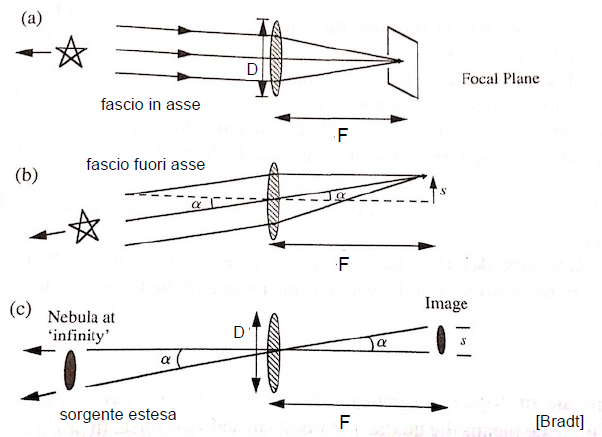
\includegraphics[width=0.49\textwidth]{Immagini/Capitolo2/Richiami_ottica_piano_focale.PNG}
	\vspace{-5pt}
	\caption*{Esempi di fasci e piano focale da sorgenti puntiformi ed estese}
	\vspace{-5pt}
\end{wrapfigure}

Facendo qualche richiamo di ottica, una lente focalizza un fascio incidente in asse con essa su un piano focale a distanza pari la lunghezza focale $F$, un fascio fuori asse di un angolo $\alpha$ verrà focalizzato a una distanza $F$ dalla lente e a una distanza $s$ dall'asse, dove:
\begin{equation*}
	s = F\tan\alpha \overset{\alpha\to0}{\simeq} F\cdot\alpha
\end{equation*}
In cui si può approsimare la tangente con l'angolo stesso per piccoli angoli. Ciò si applica alle sorgenti estese facendo combaciare il suo estremo superiore con l'asse focale e prendendo in riferimento per l'angolo $\alpha$ l'estremo inferiore, misurando in millimetri  (o in pixel tramite CCD) la distanza $s$, si trova la scala sul piano focale:
\begin{equation*}
	\frac{\Delta\alpha}{\Delta s} = \frac{1}{F}
\end{equation*}
Espressa in arcosecondi su millimetro (o su pixel), detto in inglese \textit{plate scale}(si ricordi che $\alpha$ è espresso in radianti e va convertito in arcosecondi). Si può definire una focale equivalente nota la distanza focale $F$ facendo semplicamente il rapporto tra un radiante (espresso in arcosecondi) e questa lunghezza. Un rapporto molto importante è il \textit{rapporto focale} $f$ definito come:
\begin{equation}
	\label{def:f-ratio}
	f \Def \frac{F}{D}
\end{equation}
Dove $D$ è il diametro della lente focalizzante. Questa grandezza è particolarmente importante in quanto il suo inverso $\/f$ determina la "velocità" della lente, di fatti una lente con lunghezza focale maggiore focalizzerà l'immagine su un numero di pixel $s$ maggiore a parità di angolo $\alpha$ di deviazione dall'asse, essendo le due in proporzionalità diretta. Nei tempi di esposizione, un'immagine e quindi un flusso distribuito su più pixel necessiterà di un'esposizione maggiore per avere un buono rapporto segnale-rumore, questo significa che una lente con rapporto $1/f$ piccolo, avrà lunghezza focale $F$ grande, e perciò sarà più lenta. Nel caso reale entra in gioco anche l'area collettrice, ossia le dimensioni del telescopio, le quali determinano la quantità di flusso a cui è esposto il rivelatore su cui mette a fuoco al lente. Questo significa che se un'immagine ha dimensioni lineari $s$, avrà area proporzionale a $s^2$, per cui l'energia del fotone focalizzato per ogni pixel sarà proporzionale al rapporto tra le dimensioni dell'apertura che permette il passaggio del fotone e quelle dell'immagine su cui questo fotone va a "distribuirsi":
\begin{equation*}
	E_{ph} \propto \frac{D^2}{s^2} \propto \frac{D^2}{F^2} = f^{-2}
\end{equation*}
Questo esprime che una lente con rapporto focale $f$ di piccole dimensioni, avrà grande apertura e lunghezza focale corta, per cui avrà bisogno di tempi di esposizione minori ma al tempo stesso avrà una capacità risolutiva e di distinzione degli oggetti minore, godendo però di un campo visivo (fov) maggiore, essendo l'apertura $D$ maggiore. Riassumendo, per ricordare meglio, un rapporto $f^{-1}$ piccolo corrisponde ad una piccola velocità di acquisizione, mentre un valore grande di questo parametro corrisponde a una grande velocità di acquisizione.

\begin{wrapfigure}{l}{0.5\textwidth}
	%Immagine presa da slide
	\vspace{-5pt}
	\centering
	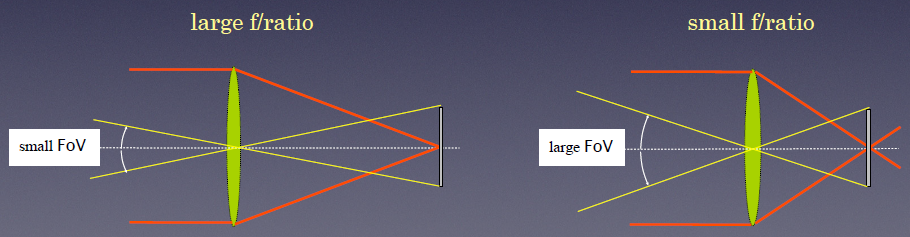
\includegraphics[width=0.49\textwidth]{Immagini/Capitolo2/fov.png}
	\caption*{Esempi di fov correlati a $f$}
	\vspace{-5pt}
\end{wrapfigure}

Un'altra proprietà collegato al rapporto focale è il \textit{campo di vista}, o \textit{fov} (field of view), proporzionale anch'esso a $f$. Di fatti, oltre che la scala sul piano focale e il tempo di esposizione, il rapporto determina per ragioni geometriche facilmente intuibili il campo di vista in modo inversamente proporzionale, per cui a un grande valore di $f$ corrisponde un piccolo campo visivo, mentre per un valore minore un campo maggiore. Correlandolo con la velocità, una lente veloce (f piccolo) avrà un campo di vista più grande, viceversa un più lenta (f grande) avrà campo di vista minore. Questo implica che le prime sono più adatte ad un'osservazione meno dettagliata ma di porzioni di cielo maggiori, mentre le seconde sono particolarmente apprezzate nella risoluzione di porzioni di cielo ed oggetti specifici. Parlando di telescopi esistenti e futuri, il telescopio POSS è stata la principale fonte di informazione per i surveys in tutto il cielo stellato fino agli anni '60, possiede $f/2.5$ e lenti correttrici, ossia è una telescopio molto veloce e ad ampio fov. Un altro esempio più recente, di inizio millennio, è il telescopio SDSS con $f/5$, per cui più lenta e precisa, che ha permesso un grande numero di scoperte nell'interstellare fino alle scale cosmologico, coprendo cinque bande nell'ottico. Attualmente in uso c'è il telescopio VISTA in Cile per il vicino infrarosso con $f/3.3$, che errà presto sostituito dal LSST entro il 2021, con $f/1.25$ (estremamente veloce e ad ampio fov). Un parametro che stima l'efficienza nella velocità di acquisizione sempre maggiore di queste macchine è il "grasp" (o "etendue" dal francese), che è l'efficienza della macchina a osservare una certa zona di cielo entro un certo flusso limite ed è definita come:
\begin{equation*}
	Grasp = D^2 \cdot FoV \, (m^2 \cdot deg^2)
\end{equation*}
Maggiore è questo parametro maggiore sarà la velocità con cui è capace di effetture osservazioni il telescopio in oggetto. Chiaramente è direttamente proporzionale al fov in quanto si tratta di un parametro osservativo, mentre tiene conto del flusso limite tramite il termine $D^2$.

\subsection*{Aberrazioni ottiche}

Sia la lente che le camere poste davanti il punto focale che costituiscono il telescopio sono fortemente influenzate degli effetti di aberrazione accennati precedentemente e che ora accenneremo più in dettaglio.

\begin{wrapfigure}{r}{0.5\textwidth}
	\vspace{-10pt}
	\centering
	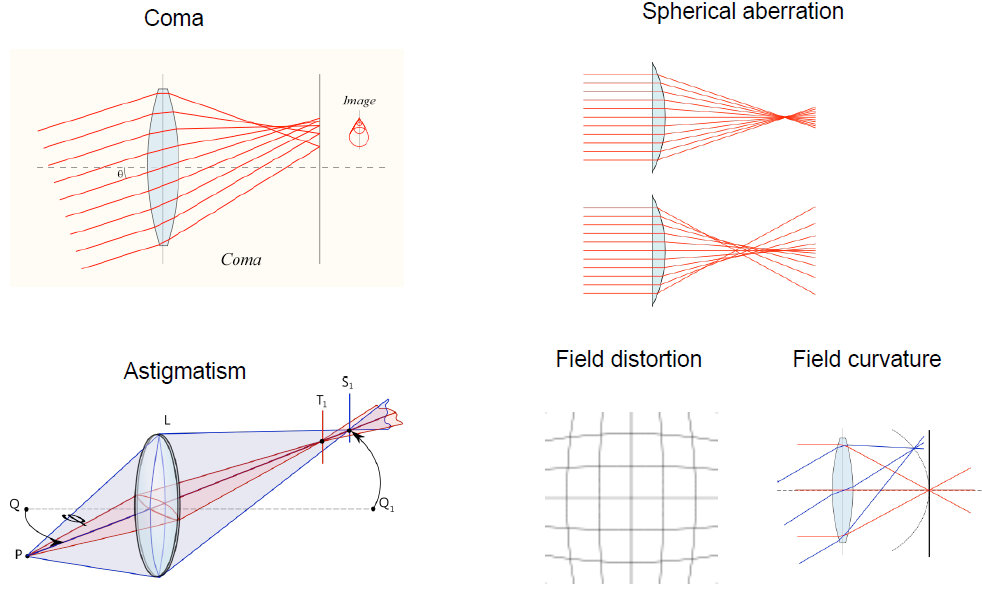
\includegraphics[width=0.49\textwidth]{Immagini/Capitolo2/Aberrazioni.png}
	\caption{Tipologie di aberrazioni ottiche}
	\vspace{-10pt}
\end{wrapfigure}

Le principali tipologie di aberrazioni ottiche, riassunte in figura, sono il \textit{coma}, l'aberrazione sferica, l'astigmatismo, la distorsione di campo e la curvatura di campo. La prima riguarda i raggi del fascio incidente più fuori asse rispetto a quelli centrali, per cui succede che per conformazione della lente convergente i corrispettivi raggi rifratti non vadano a convergere nello stesso punto, creando una piccola coda. L'\textit{aberrazione sferica} riguarda la forma della lente, per cui i raggi più distanti dall'asse ottico vengono rifratti ad angoli diversi andando a convergere in punti diversi rispetto quello focale (dove comunque confluiscono tutti i raggi che in incidenza erano più vicini l'asse). L'\textit{astigmatismo} consiste nella perdita di simmetria assiale, per cui raggi incidenti ad angoli diversi convergono a distanze focali diverse. Altri tipi di aberrazione, come quella della \textit{curvatura di campo}, procudono effetti distortivi per cui il piano focale diventa curvo, problema tipico dei telescopi a fov molto grandi e risolvibile con le moderne tecnologie creando appositi CCD curvi. Questo effetto si ritrova similmente nella \textit{distorsione di campo}, effetto che fa perdere la scala di misure del piano focale sull'intero campo di vista, come è facilmente dall'immagine, e per cui si ottengono pixel equivalenti che non hanno le stesse dimensioni costanti in tutto il campo di vista. Questi effetti possono essere limitati in principio creando strumentazioni apposite, ad esempio usando specchi parabolici anzichè sferici nei telescopi riflessivi. In generale, si parla di fov corretto per i indicare il fov di un telescopio una volta aggiunte le strumentazioni e applicate tutte quelle correzioni che puntano a ridurre gli effetti di queste aberrazioni.

% ragiona se rifare i paragrafi o mettere la prossima parte (struttura di cassegrain e telescopi riflessivi) nella parte prima delle aberrazioni o boh

\section{Telescopi riflessivi e parametri osservativi}

Il più comune dei telescopi riflessivi è il Cassegrain, citato prima, dove il fascio viene riflesso da uno specchio principale su un secondario convesso, il quale riflette a sua volta i raggi sul piano focale attraversando un buco nello specchio primario. Combinando gli effetti riflessivi dei due specchi, si può ricavare la correlazione tra le distanze focali tramite la seguente:
\begin{equation*}
	\frac{1}{F_p-d}=\frac{1}{d}+\frac{1}{F_s}
\end{equation*}
Dove $F_p$ è la distanza focale dello specchio primario, $F_s$ del secondario e $d$ la distanza a cui è interposto il secondo specchio convesso rispetto al punto focale del primo.

\begin{wrapfigure}{l}{0.30\textwidth}
	\vspace{-10pt}
	\centering
	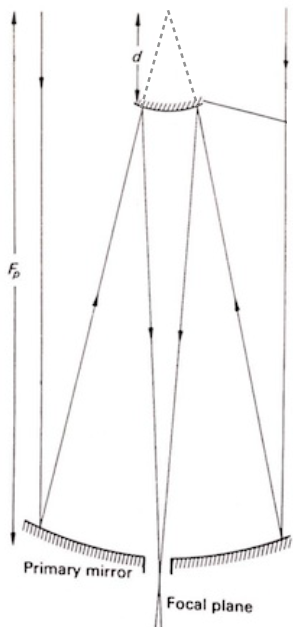
\includegraphics[width=0.29\textwidth]{Immagini/Capitolo2/Cassegrain.PNG}
	\caption{Schema del modello Cassegrain}
	\vspace{-30pt}
\end{wrapfigure}

Come accennato al paragrafo precedente, gli specchi sono parabolici per favorire la convergenza di tutti i raggi nello stesso punto focale, anche quelli maggiormente fuori asse. Lo svantaggio di questa struttura sta nell'ingombro che lo specchio secondario comporta, riducendo notevolmente il campo visivo. Un design di questa tipologia di telescopi particolarmente diffusa è quella di \textbf{Ritchey-Chrétien}, basato su strutture iperboliche per entrambi gli specchi che annullano l'aberrazione sferica e il coma, riducendo al tempo stesso l'astigmatismo e la curvatura di campo, mantenendo un fov corretto abbastanza ampio. Un altro vantaggio di questa struttura è la sua compattezza, riducendo i costi di costruzione e di sviluppo della meccanica atta a mantenerne la stabilità e a muoverlo per coprire varie parti di cielo. Il prezzo principale di questo modello è uno specchio secondario maggiore, che arriva a coprire anche il $20\%$ del campo di vista rispetto ad altri.

\subsection*{Risoluzione angolare}

Per definire il concetto di risoluzione angolare di un telescopio, è necessario fare ulteriori richiami di ottica. Un fenomeno importante ai fini della definizione di questo parametro è la \textit{diffrazione di Fraunhofer}, storicamente adoperata per la comprensione della natura della luce, se questa fosse corpuscolare o ondulatoria, il cui scopo è quello di indagare gli effetti che ha una fenditura su un fronte d'onda piano. Innanzitutto, per fronte d'onda si intendono dei punti nello spazio ugualmente distanziati in cui l'onda si trova nella stessa fase, ad esempio i fronti di picco sono quelli in cui l'onda si ritrova periodicamente ad avere dei picchi in punti ben definiti dello spazio. Una volta che questi fronti d'onda colpiscono una fenditura, quello che si osserva è la generazione di frange di interferenza costruttive e distruttive, interpretato da Fraunhofer come effetto di interferenza tra le onde che vengono generate in ogni punto della fenditura, che diventa quindi sorgente.

\begin{wrapfigure}{l}{0.45\textwidth}
	\vspace{-10pt}
	\centering
	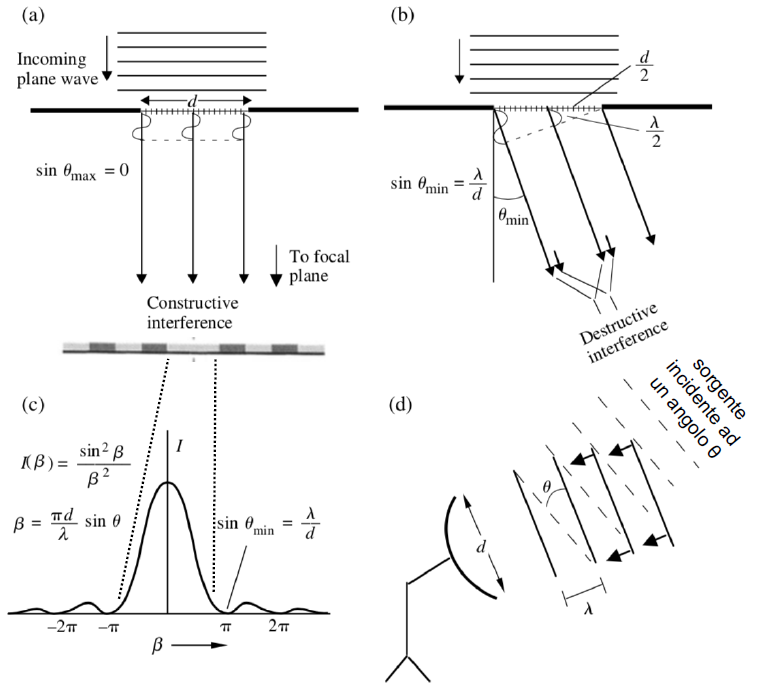
\includegraphics[width=0.44\textwidth]{Immagini/Capitolo2/Fraunhofer.PNG}
	\caption*{Diffrazione di Fraunhofer}
	\vspace{-10pt}
\end{wrapfigure}

Nel caso i fronti incidano perpendicolarmente la fenditura, le onde generate in asse saranno speculari a quelle incidenti, per cui avremmo frange ad interferenza costruttiva nelle proiezioni sul piano focale, come mostrato in figura. Nel caso la sorgente non sia in asse con la fenditura bisogna calcolare lo sfasamento di ogni fronte generato nei diversi punti di essa. Per fare questa misura bisogna considerare la differenza di cammino $\Delta s$ all'inizio della propagazione, come mostrato nella (b), tra le due onde prese in considerazione e prendendo in riferimento la congiungente ortogonale la direzione di propagazione rispetto a cui si vuole trovare l'interferenza risultante. Dalla trigonometria sappiamo che la differenza di cammino generante lo sfasamento è:
\begin{equation*}
	\Delta s = \frac{a}{2}\sin\theta
\end{equation*}
Dove abbiamo considerato le due onde come distanti metà fenditura l'una dall'altra, come nella (b), e dove $a$ è la grandezza della fenditura, $\theta$ l'angolo sotteso tra la normale alla fenditura e l'asse scelto in direzione del piano focale. Nel caso di interferenza distruttiva, le onde dovranno essere perfettamente in antifase, ossia avere una differenza di fase di $\pi$, ma essendo che le onde sono descritte da funzioni periodiche con periodo $t=2\pi$, per avere tale sfasamento dovremmo misurare una differenza di cammino pari a $\lambda/2$. Il risultato è un picco centrale luminoso seguito da zone di buio e poi nuovamente a interferenza costruttiva di dimensioni e intensità via via minori, quello che si trova per l'andamento dell'intensità di luce è:
\begin{equation*}
	I(\beta) = \frac{\sin^2(\beta)}{\beta^2} \qquad \text{dove} \,
	\beta = \frac{\pi d}{\lambda}\sin\theta
\end{equation*}
Dove chiaramente per $\theta$ nullo si ha il primo e maggiore picco, mentre per $\beta=\pi$, ossia $\sin\theta=\lambda/d$, si ha il primo minimo. Essendo i telescopi, così come anche le antenne radio e altri rivelatori, costituiti da fenditure circolari che fanno ostruzione e originano diffrazione con il segnale entrante, questo fenomeno è cruciale nella definizione di risoluzione angolare. Le sorgenti talmente vicine da avere separazione angolare vicina al rapporto tra la lunghezza d'onda del fascio incidente e il diametro del telescopio, produrranno uno sfasamento da una parte all'altra dell'entrata del telescopio (causante ostruzione). Nel caso questa differenza di percorso $\Delta s$ diventi più piccola della lunghezza d'onda stessa, non saremo più in grado di distinguere i due segnali, essendo i loro picchi di diffrazione troppo sovrapposti per essere distinguibili.

\begin{wrapfigure}{r}{0.3\textwidth}
	\vspace{-15pt}
	\centering
	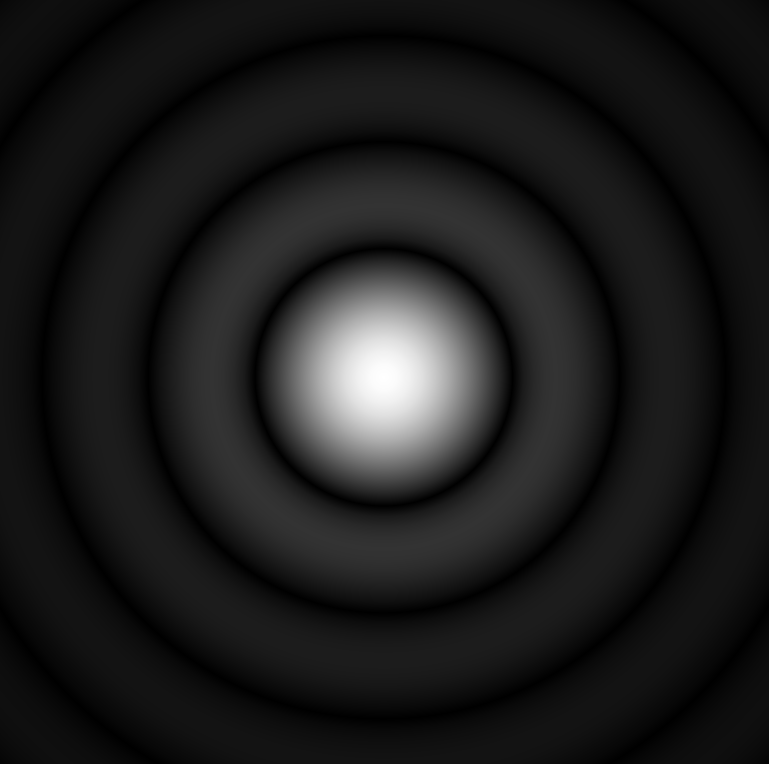
\includegraphics[width=0.29\textwidth]{Immagini/Capitolo2/Disco_Airy.PNG}
	\caption*{Disco di Airy}
	\vspace{-15pt}
\end{wrapfigure}

Risolvendo gli integrali di Wessel relativi alla fenditura circolare (caso proprio dei telescopi) viene fuori un rapporto numerico che relaziona l'angolo a cui si forma il primo minimo di diffrazione con il rapporto $\lambda/d$ tramite il fattore di forma:
\begin{equation}
	\label{eq:diff-Airy}
	\alpha_{min}=1.22\frac{\lambda}{d}
\end{equation}
Dove chiaramente il pattern di diffrazione ha simmetria circolare, anzichè la disposizione a bande analizzata prima, creando il cosiddetto \textit{Disco di Airy}. Da ciò, si introduce il concetto di \textbf{risoluzione angolare} tramite il criterio di Rayleigh, secondo cui un telescopio con apertura $d$ è in grado di risolvere due sorgenti di lunghezza d'onda $\lambda$ se esse si trovano non più vicine tra loro della distanza a cui si trova il primo minimo di diffrazione, in formula se la loro separazione angolare $\Delta\alpha$ è al massimo:
\begin{equation}
	\label{def:ris-ang}
	\Delta\alpha \Def \alpha_{min} = 1.22\frac{\lambda}{d} =
	0.12" \Bigl( \frac{\lambda}{0.5\mu m} \Bigr) \Bigl( \frac{1m}{d} \Bigr)
\end{equation}
Considerato anche il rumore di fondo presente nelle osservazioni, di norma è difficile visualizzare il secondo disco di massimo a meno che la fonte non sia particolarmente luminosa. Questo secondo picco può essere particolarmente fastidioso nel caso la rivelazione punti all'osservazione di un pianeta legato a una stella, che se posto abbastanza vicino la stella rischia di essere oscurato, in tal caso si aggiunge anche il fatto che mediamente il contrasto tra un pianeta e la propria stella è di circa un fattore dieci. 

\begin{wrapfigure}{r}{0.4\textwidth}
	\vspace{-10pt}
	\centering
	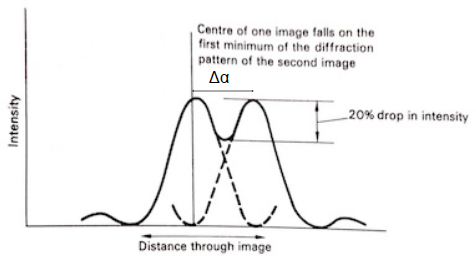
\includegraphics[width=0.39\textwidth]{Immagini/Capitolo2/Risoluzione_angolare.PNG}
	\caption{Risoluzione angolare in termini del pattern di diffrazione}
	\vspace{-5pt}
\end{wrapfigure}

Come parametro della risoluzione angolare ma anche del fit gaussiano del profilo di luminosità di una stella si usa la $FWHM$ (full width half maximum) del primo massimo di interferenza. Il discorso è più complesso per i telescopi da terra, particolarmente limitati dalla turbolenza atmosferica, mentre per quelli posti in orbita il discorso di esaurisce proprio in questi termini, dove si ricorda che la deviazione standard $\sigma$ di una gaussiana è correlata alla $FWHM$ secondo la relazione:
\begin{equation}
	\label{eq:FWHM}
	FWHM=2.355\sigma
\end{equation}
Per capire la sua importanza basta vedere il plot del pattern di diffrazione (intensità percepita sul piano focale in funzione della distanza), in cui viene rappresentato il caso limite in cui il picco della seconda sorgente cade esattamente dove si trova il primo minimo di diffrazione della prima sorgente, in questo caso le sorgenti si sovrappongono proprio nel punto di FWHM citato prima.

\subsection*{Funzione di risposta}

Pur avendo sorgenti puntiformi e ammettendo di avere risoluzione angolare inifinita come caso ideale, la fessura che il segnale deve attraversare nel telescopio crea shift di fase che portano ad un'immagine di dimensioni finite all'interno del pattern di diffrazione di Airy. Pur non trattandolo in modo rigoroso poichè servirebbero le trasformate di Fourier, otteneniamo una funzione di Bessel, che si traduce in una gaussiana smorzata. Questo discorso è importante perchè giustifica l'assunzione del valore di $\alpha_{min}$ come valore medio tipico della \textbf{point response function (PSF)}, la quale viene approssimata solo al primo massimo di interferenza con una gaussiana, mentre i secondari risultano importanti solo nella trattazione di sorgenti particolarmente luminose:
\begin{equation}
	\label{def:PSF}
	PSF \Def I_0 \Bigl( \frac{J_1(x)}{x} \Bigr)^2 \qquad
	\text{dove } x=\pi\theta \frac{D}{\lambda}
\end{equation}
Questa funzione risulta importante per fare la necessaria convoluzione del segnale in entrata dalla fenditura:
\begin{equation}
	I_{obs}(x,y)=\int_{-\infty}^{+\infty} I_{inf}(x',y')PSF(x-x',y-y')dx'dy'
\end{equation}
Empiricamente, quello che si fa è fittare una gaussiana nell'osservazione bidimensionale di una sorgente:
\begin{equation}
	PSF(r)=I(r)=I_0e^{-\frac{r^2}{2\sigma^"}}
\end{equation}
Dove la deviazione è trovata tramite la FWHM a cui è legata secondo la \ref{eq:FWHM}.

\subsection*{Seeing}

\begin{wrapfigure}{l}{0.30\textwidth}
	\vspace{-10pt}
	\centering
	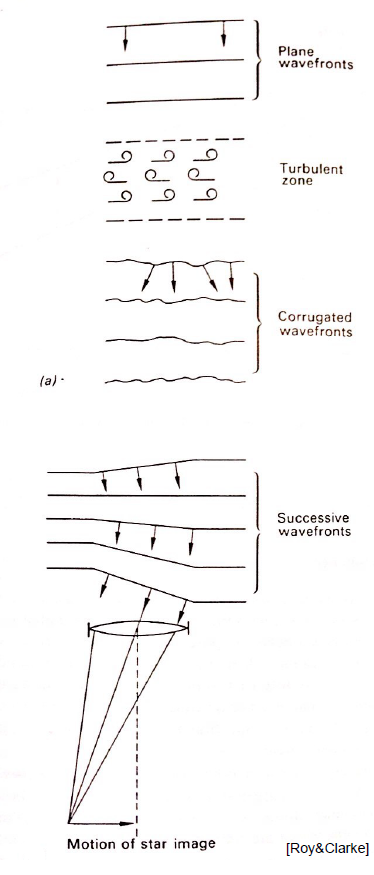
\includegraphics[width=0.29\textwidth]{Immagini/Capitolo2/Seeing.PNG}
	\caption{Effetto di seeing}
	\vspace{-10pt}
\end{wrapfigure}

Andando ad osservare una stella, il suo profilo di luce non corrisponderà al pattern di diffrazione di Airy ma avrà FWHM della gaussiana molto più larga rispetto alle dimensioni prefissate nella \ref{eq:diff-Airy}. Questo effetto è dato dalla turbolenza atmosferica ed è detto \textbf{seeing}, che affligge chiaramente i telescopi posti a terra e non quelli in orbita. Le ripercussioni dei moti convettivi atmosferici sono la creazione di bolle d'aria a temperatura e densità diverse, le quali avranno quindi indici di rifrazione diversi e il cui attraversamento da parte del segnale in arrivo dallo spazio comporta una distorsione, facendo passare i fronti d'onda originariamente piani a fronti corrugati una volta arrivati a terra. Questo comporta un effetto ottico di "danza" della sorgente attorno all'asse ottico, che si traduce in uno sfocamento dell'immagine, la quale avrà quindi una gaussiana percepita molto più larga. Per caratterizzare questo effetto si introduce il \textit{parametro di Fried} $r_0$, espresso in unità di lunghezza (tipicamente in $cm$), viene definito come il diametro dello specchio (o della lente) che rende l'immagine limitata dai soli effetti di diffrazione e l'immagine limitata di soli effetti di seeing di pari risoluzione (ossia il limite di diffrazione è equivalente a quello dato dal seeing in quello specifico sito). Alternativamente, può essere definito come il diametro dell'anello circolare su cui la radice quadratica media delle aberrazioni sul fronte d'onda dovuti al passaggio nell'atmosfera è pari a un radiante. Un valore ottimale di questo parametro è dell'ordine delle decine di centimetri, essendo che l'immagine disturbata (o meglio la gaussiana) avrà dimensioni $d_s$:
\begin{equation*}
	d_s \propto \frac{\lambda}{r_0}
\end{equation*}
Perciò tanto più questo valore sarà piccolo, maggiore sarà l'effetto di disturbo dovuta dal seeing, essendo che lo si può interpretare come dato da bolle d'aria di dimensioni minori, le quali danno maggiori effetti nella scala della microturbazioni. Viceversa, un $r_0$ maggiore, corrispondente a bolle d'aria più grandi, daranno corrugazioni su scala più ampia, disturbando di meno l'immagine. Nelle immagini limitate dal solo pattern di diffrazione, invece, le dimensioni sono date dall'apertura $D$:
\begin{equation*}
	d_s \propto \frac{\lambda}{D}
\end{equation*}
Per cui il seeing diventa dominante in caso di $r_0<D$. Si accenna che, essendo dimostrabile che $r_0\sim \lambda^{6/5}$, gli effetti di questo disturbo aumentano con l'aumentare della lunghezza d'onda, per cui in uno stesso sito gli effetti saranno maggiore al passare, ad esempio, dalla banda U alla banda K.

\begin{figure}[h]
    \centering
    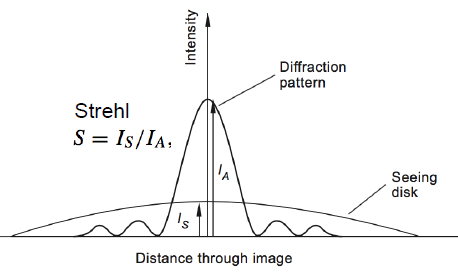
\includegraphics[width=0.45\textwidth]{Immagini/Capitolo2/Seeing_gauss_logscale.PNG}
    \caption{Effetto di Seeing in scala logaritmica rispetto all'immagine limitata da diffrazione}
    \label{im:seeing-logscale}
\end{figure}

Tutto questo discorso risulta invalidante anche per piccoli telescopi, tipicamente quelli amatoriali, per cui anche trovandosi in un ottimo sito, ma avendo un'apertura $D$ di circa mezzo metro, si trovano fortemente limitati dal disturbo atmosferico da terra. Un metodo di ricerca di siti buoni dal punto di vista del seeing, è quello di cercare posti che abbiano meno turbolenza atmosferica possibile, condizione che porta alla scelta di isole e altipiani a ovest dei continenti, essendo che l'oceano confinante funge da serbatoio a temperatura costante, che comporta l'assenza di gradienti termici e di conseguenza a un flusso laminare dei venti ad alta quota (il quale va tipicamente da ovest a est). Il caso opposto si otterrebbe scegliendo un sito su una costa orientale di un continente o un'isola, dove l'aria ha attraversato parte soprastante il suolo, il quale ha gradienti termici totalmente non costanti e per cui crea molta corrugazione nei fronti d'onda.

\begin{exrc}[Sonda Cassini e Saturno]
	La sonda Cassini, in orbita attorno Saturno da diversi anni, è finita due volte nelle condizioni geometriche tali da avere un'eclissi totale del Sole da parte del pianeta, in tal modo si sono potute fare osservazioni della lontana Terra, avendo la principale sorgente di luce del nostro sistema oscurata. Su questa sonda sono posti due telescopi, uno angolo ampio molto veloce (WAC - wide angle camera), e uno a focale maggiore e campo di vista minore (NAC - narrow angle camera), che hanno rispettivamente $F=20\, cm$ e $f/3.5$, $F=2\, m$ e $f/10.5$, mentre i CCD danno pixel di $12\, \mu m$. Ora la distanza di Saturno in quell'istante era $d=1.44\e{12}m$, mentre la distanza tra la Terra e la Luna media è $T-L=3.84\e{8}m$. Si chiede di trovare:
	\begin{enumerate}
		\item Qual è la scala in arcsec/pixel in WAC e NAC?
		\item Quanti arcsec (e pixel) separano la Terra dalla Luna nelle immagini WAC e NAC?
		\item Risoluzione angolare di WAC e NAC
		\item La Terra e’ risolta nelle immagini ?
	\end{enumerate}
\end{exrc}

\begin{sol}
	Suddividiamo la soluzione nei rispettivi punti posti nell'esercizio, chiamando $C=206265$ il fattore di conversione tra arcosecondi e radianti:
	\begin{enumerate}
		\item Scala in arcsec/pixel in WAC e NAC (il fattore di conversione da millimetri a pixel è dato dalle dimensioni del CCD $1mm / 12\mu m = 83 \,pixel / mm$):
		\begin{itemize}
			\item Scala WAC: $\frac{C}{F}=\frac{206265}{200mm}=1031"/mm=12.4"/pxl$
			\item Scala NAC: $\frac{C}{F}=\frac{206265}{2000mm}=103.1"/mm=1.2"/pxl$
		\end{itemize}
		\item Separazione Terra-Luna nei due telescopi:
		
		$
		\theta(T-L)=\frac{T-L}{d}\cdot C=\frac{3.84\e{8}m}{1.446\e{12}m}\cdot 206265=54.8"=
		\begin{cases}
			4.4 \, pxl \quad \text{WAC} \\
			45 \, pxl \quad \text{NAC}
		\end{cases}
		$
		\item Risoluzioni angolari di WAC e NAC (si tralascia il calcolo di $D$ in quanto di derivazione diretta da $F$ e $f$ sfruttando la \ref{def:f-ratio}):
		
		$
		\alpha=0.12"\frac{\lambda}{0.5\mu m}\frac{1m}{D(m)}=
		\begin{cases}
			0.12"\frac{1}{0.057}=2" \quad \text{WAC} \\
			0.12"\frac{1}{0.19}=0.6"\quad \text{NAC}
		\end{cases}
		$
		\item Affinchè la Terra venga risolta da entrambi i telescopi, è necessario che abbia dimensioni maggiori della risoluzione angolare:
		
		$
		\theta(Terra)=\frac{2R_T}{d}\cdot C=\frac{2\cdot 6.371\e{6}m}{1.446\e{12}m}\cdot 206265=1.8"
		\begin{cases}
			\text{WAC non risolve la Terra} \\
			\text{NAC risolve la Terra}
		\end{cases}
		$
	\end{enumerate}
\end{sol}

\begin{exrc}[Terra vista da Marte]
	A bordo	della sonda Mars Reconnaissance Orbiter in orbita attorno a Marte c'è un piccolo telescopio di nome HIRISE, con diametro del riflettore $D=0.5\, m$, lunghezza focale $F=12\, m$ e la cui grandezza dei pixel è $pxl=12\, \mu m$, il cui compito è l'osservazione e la mappatura del suolo marziano. La camera venne disegnata affinchè ad ogni pixel corrispondesse un metro di suolo marziano in base alla distanza a cui questo telescopio orbitasse, e per fare osservazioni nella banda del visibile. Un giorno questa camera venne rivolta per curiosità verso la Terra e la Luna, per cui è come se fossimo nei panni di un osservatore amatoriale che rivolge il proprio sguardo verso Marte. Come riferimento, nell'istante in cui l'osservazione della Terra da parte di HIRISE venne fatta la distanza Terra-Marte (molto variabile) era $d=2.06\e{8}\, m$. Si chiede di calcolare:
	\begin{enumerate}
		\item Dimensioni angolari della Terra
		\item Diametro necessario al telescopio per risolvere l'Italia
	\end{enumerate}
\end{exrc}

\begin{sol}
	Suddividiamo la soluzione nei rispettivi punti posti nell’esercizio, chiamandoC=206265il fattore di conversione tra arcosecondi e radianti:
	\begin{enumerate}
		\item Per il calcolo delle dimensioni angolari della Terra, è sufficiente prendere il suo diametro e rapportarlo con la distanza da cui viene osservato, per poi convertirlo in arcosecondi rispetto quell'osservatore:
		\begin{itemize}
			\item $\theta(Terra)=\frac{2R}{d}\cdot C=\frac{2\cdot 6.371\e{6}m}{2.06\e{8}m}\cdot 206265=10.6"$
			\item  $\theta(Luna)=\frac{2R}{d}\cdot C=\frac{2\cdot 1.737\e{6}m}{2.06\e{8}m}\cdot 206265=3.5"$
		\end{itemize}
		\item L'Italia, essendo lunga all'incirca $2\e{6}m$, avrà un'estensione angolare di due arcosecondi, per risolverla sarà necessaria quindi una risoluzione doppia rispetto le sue dimensioni angolari per via della diffrazione (numericamente la metà della sua estensione - $1"$) e il telescopio necessiterà quindi di un diametro di apertura:
		
		$D=\frac{0.12"}{1"}=0.12m$
		
		Dove si è sfruttata la definizione di risoluzione angolare \ref{def:ris-ang} per il calcolo, adottando un segnale di lunghezza d'onda pari a mezzo micron, compatibile con il fatto che si stia facendo osservazioni nella banda del visibile. Ma essendo che HIRISE ha $D=0.5m$, ha risoluzione $0.12/0.5=0.2"$ e riesce quindi a risolvere bene i dettagli sulla Terra nel visibile. Si ricorda che per calcolare il pixel scale si usa:

		$pixel \, scale = \frac{C}{F(mm)}\frac{1}{pxl/mm}$

		Da cui otteniamo $206265/12\e{3}mm/83=0.2"$ per HIRISE.
	\end{enumerate}
\end{sol}

\section{Ottiche adattive}

Nel cercare di risolvere il problema della distorsione data dagli effetti di seeing si introducono mezzi in grado di analizzare il fronte d'onda ancora prima che esso venga convogliato sul piano focale, detti \textit{ottiche adattive}. Una di queste può essere quella rappresentata nella figura \ref{im:ottiche-adattive}, in cui un sistema di controllo possibile è dato da una serie di specchi, di cui uno adattivo, che cerca di rimodellare il fronte d'onda corrugato in entrata in modo tale da renderlo nuovamente piano. Lo specchio adattivo è costituito a sua volta da tanti piccoli specchi in grado di adattarsi al fronte d'onda corrugato.

\begin{figure}[h]
	\centering
	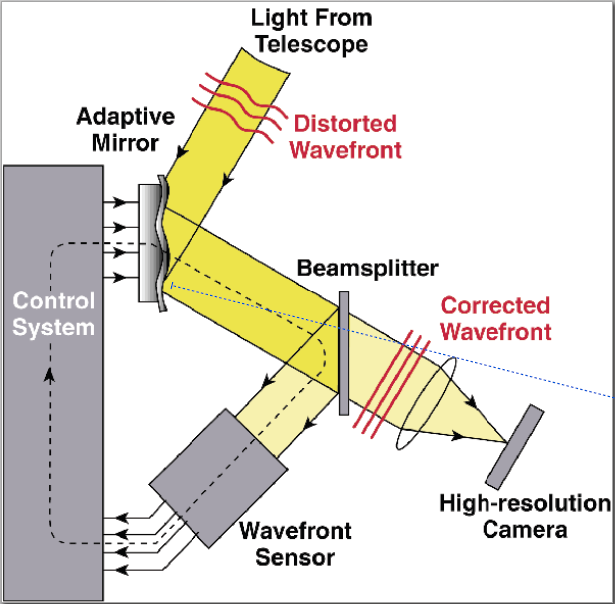
\includegraphics[width=0.5\textwidth]{Immagini/Capitolo2/ottiche_adattive.PNG}
	\caption{Schematizzazione di ottiche adattive}
	\label{im:ottiche-adattive}
    \vspace{-5pt}
\end{figure}

Il sensore di analisi dei fronti d'onda, il cui modello di riferimento è lo \textit{Shack-Hartmann}, è ciò che caratterizza il fronte entrante e applica correzioni alle distorsioni date dalla turbolenza atmosferica. Esso si costituisce di un sistema ottico composto di molte lenti di piccole dimensioni, attraverso il quale si lascia passare il segnale, e di un CCD posto oltre questo sistema; solitamente queste lenti sono sull'ordine della decina di centimetri in modo da essere paragonabili alle celle convettive che in atmosfera danno gli effetti di seeing. Nel caso il fronte incidente sia piano, le immagini focalizzate (limitate dalla sola diffrazione grazie alla scelta di lenti piccole) saranno disposte simmetricamente così come lo sono le lenti, come nel primo esempio riportato in figura \ref{im:sensore-Shack-Hartmann}. Chiaramente nel caso reale il fronte è corrugato, ed ogni lente focalizza parte di questo fronte in un punto diverso rispetto quello tracciato dall'asse focale, in quanto una corrugazione è equivalente al ricevere un segnale inclinato rispetto il piano focale.

\begin{wrapfigure}{r}{0.4\textwidth}
	\centering
	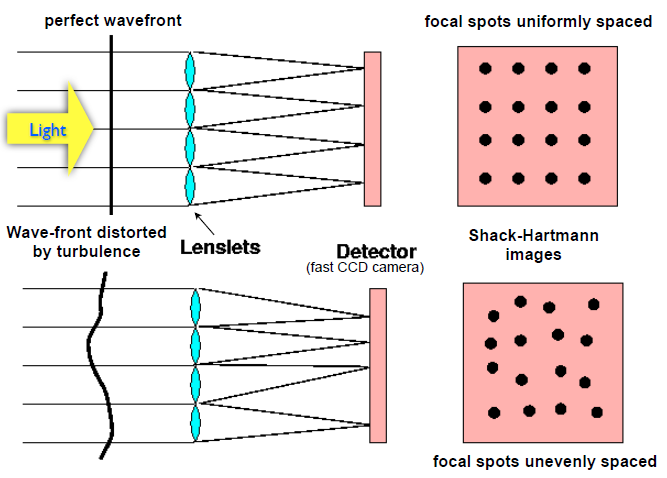
\includegraphics[width=0.39\textwidth]{Immagini/Capitolo2/sensore_Shark_Hartmann.PNG}
	\caption{Schema sensore Shark-Hartmann}
	\label{im:sensore-Shack-Hartmann}
	\vspace{-10pt}
\end{wrapfigure}

La presenza del CCD permette di rilevare la traslazione che le immagini hanno rispetto alla griglia delle lenti, tramite elaborazione software di queste rilevazioni si è così in grado, tramite il sistema di controllo, di calcolare e attuare le necessarie correzioni allo specchio adattivo in modo che il fronte torni ad essere approssimativamente piano. Questo tipo di sensore ha come condizione limitante la necessità di un flusso entrante non indifferente, essendo che il segnale viene separato e focalizzato da diversi specchi. Grazie allo sviluppo recente in ambito software e hardware, queste rilevazioni e correzioni vengono attuate ogni decimo di secondo e coprono un arco di pochi millisecondi. Questa tecnica è utilizzabile con tutte le fonti osservate una volta determinato l'adattamento ottico da usare in una determinata zona di cielo, ma essendo che le stelle luminose necessarie a questo metodo di ricerca sono molto poche, per molte zone di cielo si ricorre a stelle artificiali. Queste vengono simulate da dei laser puntati da terra verso la direzione del campo di vista, i quali sono appositamente a lunghezze d'onda di emissione del sodio, come ad esempio a $\lambda=5890\angstrom$.

\begin{wrapfigure}{l}{0.4\textwidth}
    \centering
    \vspace{-5pt}
    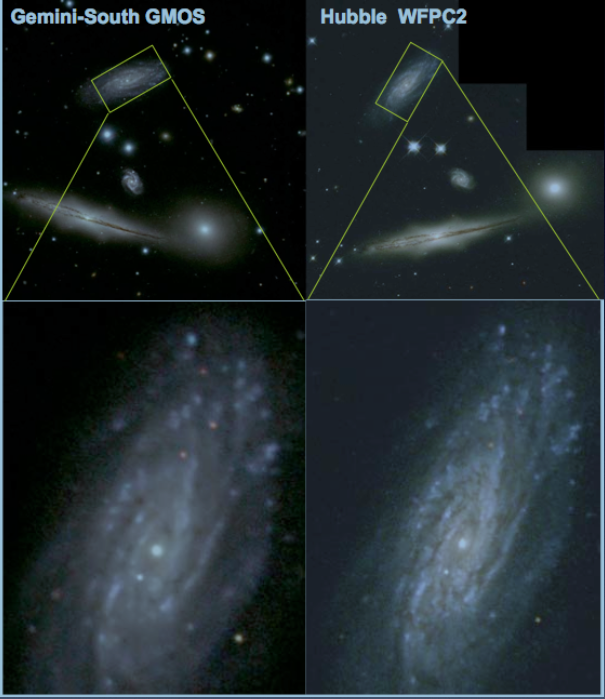
\includegraphics[width=0.39\textwidth]{Immagini/Capitolo2/Seeing_vs_Hubble.PNG}
    \caption{Comparativa tra immagine corretta e immagine presa da telescopio in orbita (Hubble space telescope)}
    \label{im:seeingvsHubble}
    \vspace{-5pt}
\end{wrapfigure}
 
Questa scelta deriva dal fatto che a circa $80\, km$ da terra c'è un piccolo strato di sodio ed eccitarlo tramite l'utilizzo di laser crea uno spot luminoso nel cielo che funge da metro di calcolo dell'ottica adattiva. Questo non è un simulatore perfetto di una sorgente cosmica in quanto non si trova a distanza infinita, ma risulta comunque al di sopra di un'ottima fetta di atmosfera. Questa tecnica permette di recuperare una buona parte di risoluzione limitando notevolmente gli effetti atmosferici, ovviamente non tanto da tornare al caso in cui l'unica limitazione sia quella imposta da diffrazione, come si vede nella figura \ref{im:seeingvsHubble}, dove si propongono immagini dello stesso oggetto ma una presa da terra tramite ottiche adattive e una dal telescopio Hubble in orbita. Ciò che fanno queste ottiche adattive, pensando in senso più tecnico, è schiacciare il cerchio di interferenza del seeing al di sotto dei minimi di diffrazione, come si vede nell'immagine \ref{im:seeing-logscale}. Il caso reale corrisponderà a una gaussiana sufficientemente piccata di dimensioni $\sim \lambda/D$, che costituirà il nucleo fondamentale dell'immagine, circondata da un alone di interferenza di dimensioni date dal seeing $\sim \lambda/r_0$. Per quantificare quanto sia buona un'ottica adattiva si introduce il parametro \textit{Strehl}, definito come il rateo tra il picco di intensità del core ottenuto rispetto all'alone sul picco ideale di intensità nel caso di sistema ottico perfetto. Nel caso di buone ottiche, questo valore sta a circa $0.6$ e $0.7$. I risultati migliori con queste ottiche si ottengono chiaramente, oltre che a lunghezza d'onda maggiori e in siti con un buon seeing, per sorgenti particolarmente luminose e soprattuto zone di cielo in cui le sorgenti siano separate e distinte, che di per sè non diano un alone luminoso, come può succedere con alcune nebulose. Per le caratteristiche del seeing, queste ottiche con laser sono un mezzo fondamentale adottato in ogni telescopio gigante, affinchè la loro altissima risoluzione non venga limitata dal seeing, e che continueranno ad essere parte integrante anche dei futuri telescopi.

\subsection*{Telescopi moderni}

\begin{wrapfigure}{l}{0.35\textwidth}
    \centering
    \vspace{-10pt}
    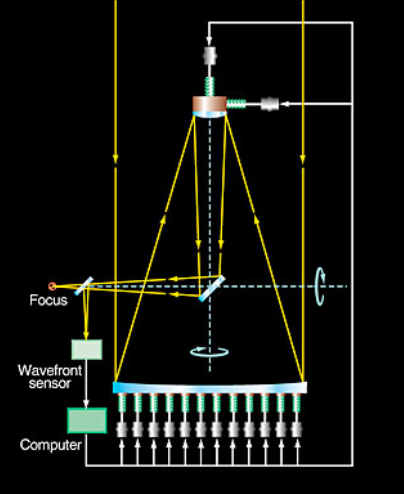
\includegraphics[width=0.34\textwidth]{Immagini/Capitolo2/Struttura_telescopio_ESO.PNG}
    \caption{Struttura telescopi ESO}
    \label{im:struttura-ESO}
    \vspace{-10pt}
\end{wrapfigure}

I telescopi moderni, di dimensioni sempre maggiori, sono soggetti a un effetto di allontanamento dell'immagine dal piano focale, unitamente a una serie di distorsioni. Ciò è dovuto a diveri fattori, come la deformazione degli specchi sempre più grandi e pesanti sotto la forza peso, oppure la loro dilatazione termica dovuta al surriscaldamento dell'impianto. Per evitare questi effetti, si è iniziati a costruire specchi sempre più sottili e leggeri (oggigiorno sono spessi circa $20cm$), abbinati ad un sistema meccanico di pistoni che regolino l'inclinazione dello specchio principale (o meglio, della serie di specchi che lo costituisce), in modo da ridurre al minimo questo tipo di aberrazioni. Anche questo metodo può essere considerato di ottica adattiva, si differenzia per l'agire direttamente sullo specchio primario. Uno dei siti di osservazione più famosi al mondo ed estremamente usato dalla comunità scientifica europea è lo Euopean Southern Observatory (ESO), collocato in Chile a Cerro Paranal, dove sono situati 4 dei telescopi più costosi al mondo, la cui risoluzione angolare arriva fino a cinque centesimi di arcosecondo, riuscendo a rilevare oggetti fino a magnitudine $27$ in un'ora di integrazione (ossia esposizione). Questi telescopi hanno struttura Ritchey-Chrétien, con uno specchio semitrasparente inclinato di $45^{\circ}$ posto al centro tra lo specchio primario e quello secondario: in tal modo si possono ricavare due ulteriori fuochi oltre quello Cassegrain, detti \textit{fuochi di Nasmyth}, in cui poter allocare altri sensori al di fuori del principale, come mostrato nella \ref{im:struttura-ESO}. L'ESO include anche telescopi ausiliari di un paio di metri con il compito di tenere in fase i quattro telescopi più massivi in modo da creare un telescopio equivalente di $100\, m$, compito estremamente arduo. Oltre a questi ci sono anche altri telescopi di varia natura di cui uno di circa due metri e mezzo fatto completamente dall'Italia. Questa combinazione di telescopi è utile come complemento alle osservazioni in orbita, principalmente fornite dal celebre Hubble Space Telescope (HST), che campiona il cielo con operazioni di imaging molto accurate, mentre il lato di analisi spettroscopica viene lasciato più frequentemente ai telescopi a terra. Un altro telescopio che collabora in orbita con il HST è Andromeda, il cui nome tecnico è M31, anch'esso a struttura Ritchey-Chrétien con rateo focale molto alto e che fa imaging dall'ultravioletto fino al vicino infrarosso (banda H), oltre il NIR si avrebbe un rumore troppo grande nelle osservazioni per via dell'emissione termica terrestre(come corpo nero). Tutti questi telescopi danno poi, nella risoluzione dei singoli oggetti, un mosaico di immagini in grado di descrivere l'intera galassia. Un altro telescopio degno di nota è il Keck Telescope, di fine anni $'90$, che rappresenta lo stacco dalle strutture monolitiche degli specchi principali, i quali arrivano fino a $8\, m$, per intraprendere una tecnica a mosaico, questo in particolare è un telescopio di $10\, m$ costituito da $36$ specchi esagonali opportunamente orientati.

\begin{wrapfigure}{r}{0.5\textwidth}
    \centering
    \vspace{-10pt}
    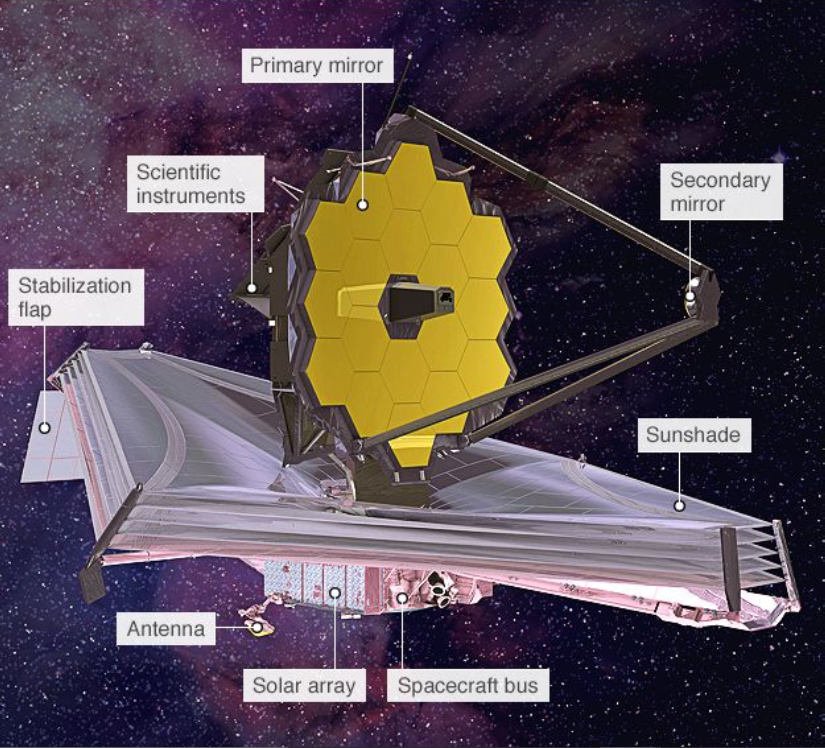
\includegraphics[width=0.49\textwidth]{Immagini/Capitolo2/Jamews_Webb_ST.PNG}
    \caption*{Rappresentazione del James Webb Space Telescope}
    \vspace{-10pt}
\end{wrapfigure}

Un altro esempio di struttura a composizione esagonale dello specchio primario è data dal futuro James Webb Space Telescope, il quale avrà un principale da $6.6\, m$ costituito da $18$ segmenti e che lo renderà il telescopio più grande in orbita attorno alla Terra (HST è $2.2\, m$), e che dovrebbe essere lanciato nell'estate del 2021. La difficoltà sta chiaramente nel compattare tutte le sue componenti, all'interno del razzo che verrà lanciato, tra le quali gli specchi e i vari strati laminari che comporrano la schermatura dei rivelatori rispetto al sole. Questo telescopio avrà due camere per l'imaging e uno spettrografo, più una camera dotato di entrambi, tutto abbastanza specifico all'indagine nel vicino infrarosso. Essendo che la banda interessata è il NIR, nonostante le grandi dimensioni del telescopio le misurazioni saranno fortemente limitate da diffrazione, essendo che per la definizione \ref{def:ris-ang} una lunghezza d'onda maggiore comporta una risoluzione minore, arrivando nello specifico ad avere una risoluzione teorica di $2\mu m$ (leggermente inferiore rispetto HST). Si ricorda inoltre che in quella banda c'è un rumore di fondo molto forte dato dall'emissione termica terrestre. Nonostante ciò, il telescopio è stato ideato appositamente per studiare quella banda, in quanto per via degli effetti di redshift è proprio in essa che ricadono i corpi celesti più distanti e antichi, che conferiscono per cui tutta questa importanza a queste lunghezze d'onda. Un alro telescopio che farà da riferimento per le successive strutture giganti è lo European Extremely Large Telescopes (E-ELT), un telescopio gigante da $39\, m$ a specchi segmentati, con $5\, m$ di specchio secondario e anche un terzo e quarto specchio adattivo per ottenere il massimo della risoluzione possibile. Questo sarà un po' un tuttofare delle rivelazioni (posto chiaramente a terra), includendo anche spettrografi in grado di analizzare anche corpi a grande distanza. Chiaramente, i telescopi in orbita richiedono manuntezione così come quelli a terra, per cui sono necessarie missioni periodiche che correggano eventuali errrori negli specchi tramite lenti correttrici (una sorta di occhiali), così come l'aggiornamento dei CCD delle camere o direttamente la sostituzione dei rivelatori con tecnologie più aggiornate dove necessario, come sistemi elettronici e giroscopi.

\subsection*{Rapporto segnale-rumore}

In qualsiasi ambito della fisica, ogni misura consiste nel rivelare una quantità che sia sufficientemente piccata rispetto alle fluttuazioni del rumore, il quale può essere di varia natura, cosa che si ritrova anche in ambito astrofisico. La miurazione in astrofisica sperimentale può essere anche di imaging, così come di spettroscopia o altro ancora, e il rumore può derivare, come visto, da sorgenti esterne non interressanti ai fini dell'osservazione, così come dall'elettronica stessa adoperata. Quest'ultima, con lo sviluppo tecnologico, è diventata man mano fonte di disturbo sempre minore, parallelamente all'aumento della precisione con cui svolge le misurazioni. Quando si parla di rumore di fondo si intende specificamente quello dato dal cielo, anch'esso è soggetto a fluttuazione come ogni tipo di rumore, che varia a seconda del sito e della regione in cui si fanno le osservazioni, ed è dato dalla luminosità del cielo, essendo che le misurazioni in questo ambito sono essenzialmente di cattura e assorbimento di fotoni in determinate bande.

Chiamiamo $C$ il numero di fotoni del segnale raccolti in un certo tempo di integrazione, o per meglio dire il numero di conteggi dei fotoni una volta passati attraverso l'ottica e rivelati con una determinata efficienza dal CCD (una volta si adoperavano fotomoltiplicatori). Con lo stesso tipo di discorso si definisce anche il numero di fotoni $B$ dato dal background (o fondo) nel medesimo intervallo di tempo di acquisizione, per cui il segnale totale sarà dato dalla somma dei due. Ora, il conteggio dei fotoni segue la statistica di Poisson, dove se $m$ è il numero medio di conteggio in un periodo di integrazione $T$, la probabilità di avere $x$ fotoni nell'intervallo $T$ è:
\begin{equation}
    P(x)=m^xe^{-\frac{m}{x^2}} \qquad \text{con } \sigma^2=m
\end{equation}
Dove $\sigma^2$ è la varianza e coincide con il conteggio medio. Questa statistica è tipica delle esperienze di conteggio e per questo descrive sia $C$ che $B$. Il problema ora si sposta nell'isolare e misurare separatamente queste due quantità, le quali chiaramente arrivano insieme e indistintamente al nostro telescopio. Un metodo può essere quello di acquisire in una regione del cielo "vuota", da cui riusciamo ad ottenere una stima del fondo $E_{est}$, per poi ottenere il segnale pulito sottraendolo ai conteggi: $S=(C+B)-B_{est}$. Chiaramente, il conteggio dei fotoni in un certo intervallo di tempo, come vedremo, sarà direttamente proporzionale al suo flusso emittente tramite costanti di proporzionalità come l'area collettrice di questi fotoni e la sua efficienza nel rivelarli. Essendo questa quantità una combinazione lineare di altre grandezze soggette tutte alla statistica poissoniana, la varianza di $S$ sarà data per propagazione dalla somma delle varianze, ponendo $B=B_{est}$ otteniamo l'errore tramite la radice quadrata della varianza:
\begin{equation*}
    \sigma_S=\sqrt{C+2B}
\end{equation*}
Grazie a questo definiamo il \textbf{rapporto segnale-rumore} (signal-noise) $S/N$ come il rapporto fra il segnale della sorgente rivelato e le fluttuazioni a cui è soggetto:
\begin{equation}
    \label{def:sig-noise}
    \frac{S}{N} \Def \frac{C}{\sigma_S} = \frac{C}{\sqrt{C+2B}}
\end{equation}
Poste le quantità in unità di tempo come $c_s$ il rateo di conteggio del segnale e $c_b$ il rateo di conteggio del fondo, in un tempo di integrazione $T$ la \ref{def:sig-noise} diventa:
\begin{equation*}
    \frac{S}{N} = \frac{c_sT}{\sqrt{c_sT+2c_bT}} \propto
    \begin{cases}
        \sqrt{c_sT} & C \gg B \quad \text{caso limitato dal segnale}\\
        \frac{c_s}{\sqrt{2c_b}}\sqrt{T} & C \ll B \quad \text{caso limitato dal rumore}
    \end{cases}
\end{equation*}
Interessante è la proporzionalità diretta con il tempo di integrazione, questo rapporto sancisce che a parità di qualità del segnale si può ottenere un rapporto $S/N$ migliore con un tempo di integrazione maggiore. Si nota inoltre che i parametri di flusso $c_x$ hanno una dipendeza intrinseca con l'area collettrice $D^2$, poichè determina la quantità di flusso misurabile, da ciò si deduce una dipendenza lineare con l'apertura del telescopio $D$ (essendo che i parametri di flusso sono sotto radice).

\subsection*{Flusso limite}

Un concetto molto importante nell'astronomia moderna è quello di \textbf{flusso limite}, con cui si intende il flusso minimo per cui con un determinato sistema ottico e con un certo tempo di integrazione risulta ancora rivelabile una sorgente dal telescopio. L'importanza di questa grandezza risiede nell'interesse che si ha nell'osservare gli oggetti più deboli e lontani, e conseguentemente adattare i progetti e i telescopi a seconda degli obiettivi che si vogliono raggiungere. Ricordando l'equivalenza tra parlare di flussi, magnitudini o conteggi (come si è fatto nel paragrafo precedente), questo parametro è anche detto \textbf{magnitudine limite}, dal momento che:
\begin{equation*}
    mag=-2.5\log{Counts}+ZeroPoint
\end{equation*}
Si adoperano inizialmente sorgenti deboli e note vicino al sito che si vuole osservare, tramite di esse si operano delle correzioni di calibrazione che andranno poi nello $ZeroPoint$, grazie a queste sarà poi possibile effettuare una buona stima della magnitudine di un oggetto ignoto. Come flusso minimo associabile ad una sorgente si prende un rapporto $S/N=3$, il quale equivale a parlare di rivelazioni di $3\sigma$, sotto questo valore non possiamo affermare con buona probabilità che si tratti di una sorgente piuttosto che di una fluttuazione del rumore di fondo. Nel caso si tratti di una sorgente particolarmente luminosa o il tempo di esposizione sia sufficientemente elevato, quando il numero di conteggi tende a infinito la poissoniana è approssimabile da una gaussiana nella trattazione statistica. Cercando di tradurre tutto ciò in termini matematici, definendo il flusso limite rilevabile come $S/N=\gamma$, otteniamo dalla \ref{def:sig-noise}:
\begin{equation*}
    C^2-\gamma^2C-2\gamma^2B=0
\end{equation*}
Il flusso limite sarà propozionale al rateo di conteggi limite $c_{s,lim}$, dove ricordiamo che $c_s=C/T$, $c_b=B/T$:
\begin{equation*}
    c_{s,lim} = \frac{1}{T} \Biggl( \frac{\gamma^2}{2}+\gamma\sqrt{\frac{\gamma^2}{2} + 2c_bT} \Biggr)
\end{equation*}
